\documentclass[times, utf8, seminar]{fit}

%\batchmode
%\usepackage{booktabs}
\usepackage{listings}
\usepackage{longtable}
\usepackage{xcolor}
\usepackage{float}
\usepackage{enumitem}
\usepackage{hyperref}

\begin{document}

\title{Analiza poslovnih podataka sa "open source" software-om}

\author{Ernad Husremović}
\brindex{DL 2792}
\verzija {1.9.7}

\mentor{prof.dr Vanja Bevanda}

\maketitle

\tableofcontents

\chapter{Uvod}

\section{BI Pojmovi}

\subsection{ETL}

\subsection{Ulazni podaci - ERP podaci}

\chapter{OLAP Case study: Analiza podataka `F18 knowhow' ERP-a}

\begin{figure}[H]
\centering
\includegraphics[width=15cm]{img/F18_erp.png}
\caption{ERP aplikacija, F18 klijent}
\end{figure}

Operativni podaci `F18 knowhow' smješteni su u ovaj relacijski model:

\begin{figure}[H]
\centering
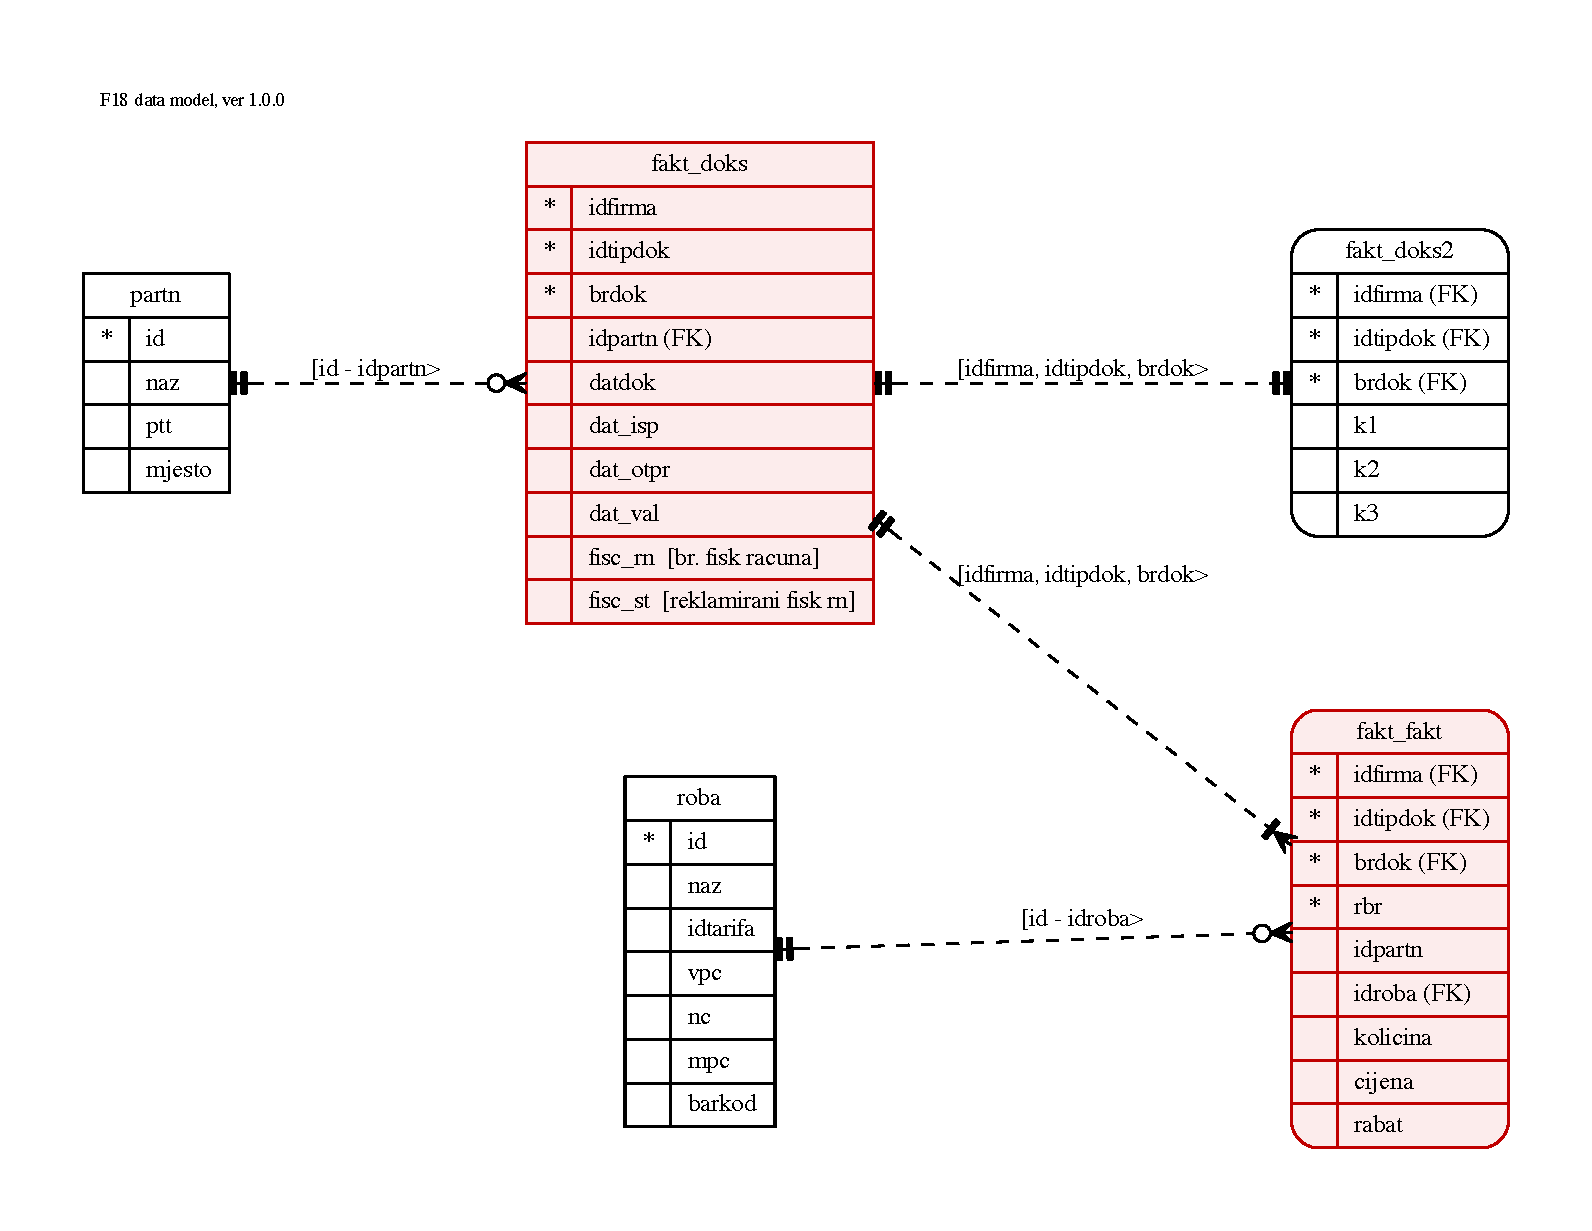
\includegraphics[width=15cm]{img/F18_db.pdf}
\caption{F18 transakcijski db model (relevantni dio)}
\end{figure}

Podaci svake poslovne godine nalaze se u posebnoj PostgreSQL bazi podataka.

Cleansing

F18 `cleansing' podaci  (Dodatak \ref{chap:izvorni_kod}, olap\_cleansing `spreadsheet' dokument)

Klasificiranje izvornih podataka - šifrarnik artikala

\begin{figure}[H]
\centering
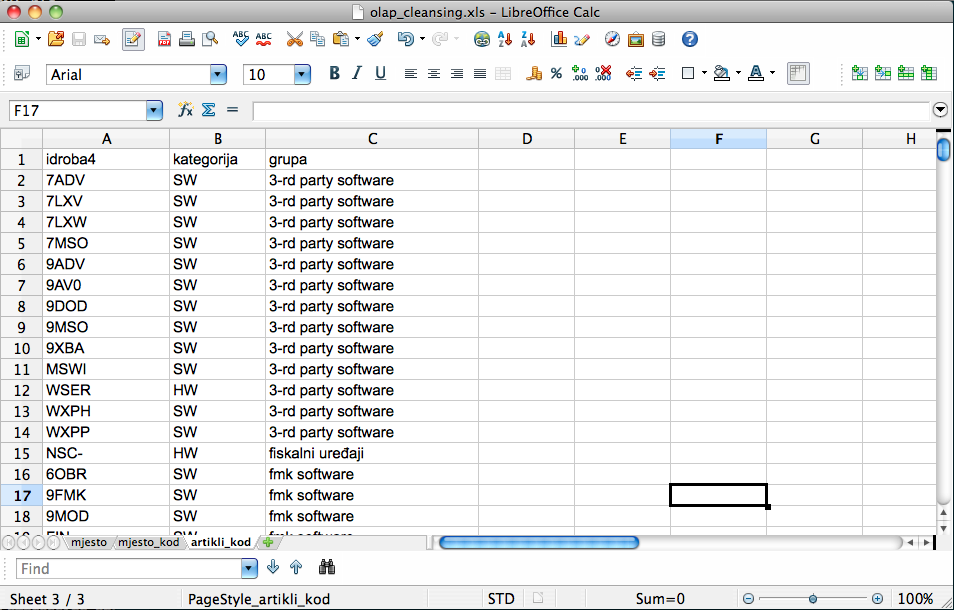
\includegraphics[width=15cm]{img/clean_artikli.png}
\caption{F18 klasificiranje - šifarski sistem artikala}
\end{figure}



\begin{figure}[H]
\centering
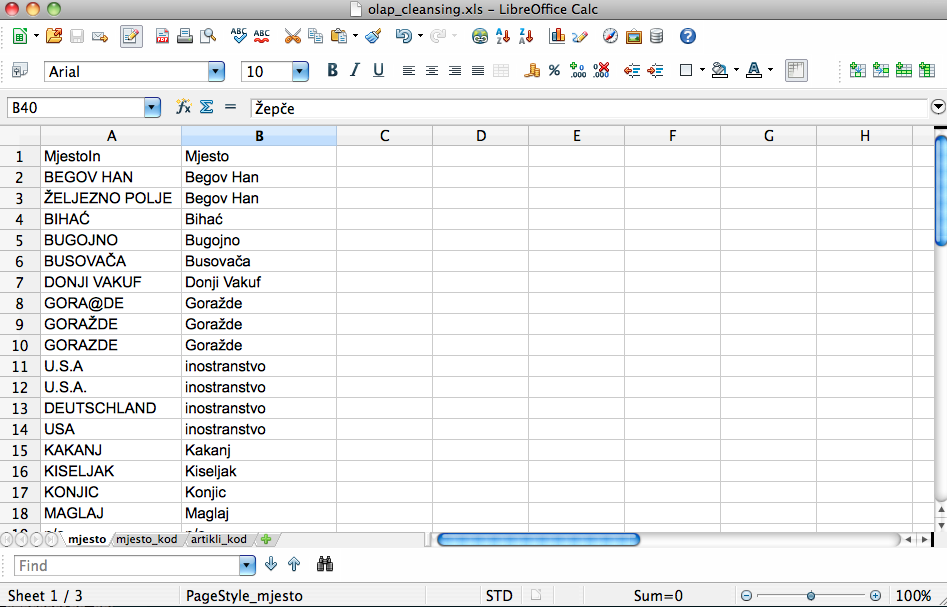
\includegraphics[width=15cm]{img/clean_mjesto.png}
\caption{`cleansing' F18 podataka -  klijenti - mjesta/gradovi}
\end{figure}


\begin{figure}[H]
\centering
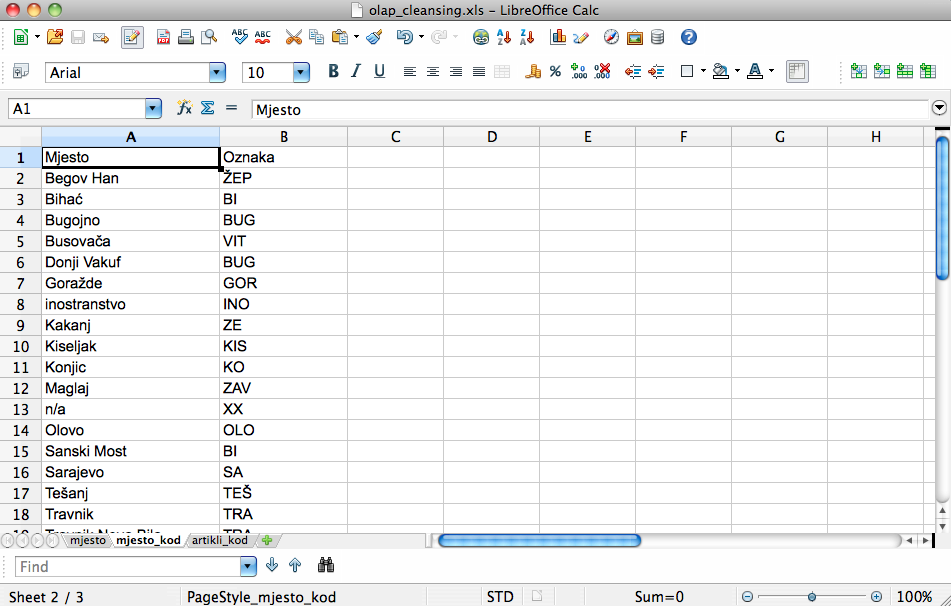
\includegraphics[width=15cm]{img/clean_mjesto_region.png}
\caption{F18 kodiranje regiona - klasifikacija mjesta/gradova}
\end{figure}


\begin{figure}[H]
\centering
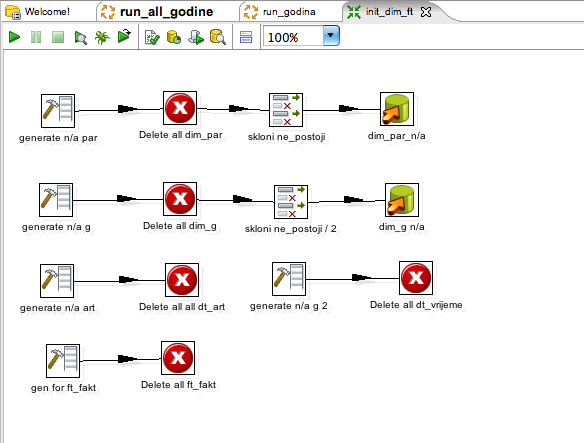
\includegraphics[width=15cm]{img/kettle_tr_init_dim_fpt.png}
\caption{Inicijalizacija `dimension' i `facts' tabela}
\end{figure}


\begin{figure}[H]
\centering
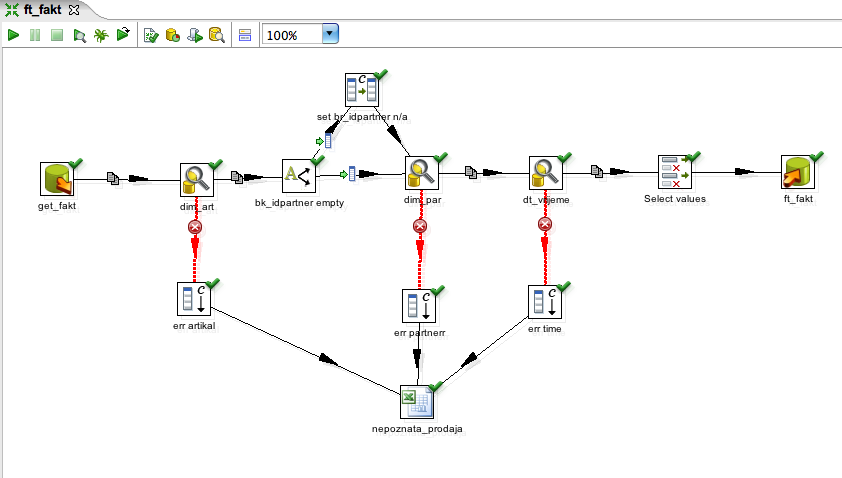
\includegraphics[width=15cm]{img/kettle_tr_ft_fakt.png}
\caption{Generacija "ft\_fakt" `facts' tabele za određenu poslovnu godinu}
\end{figure}


\begin{figure}[H]
\centering
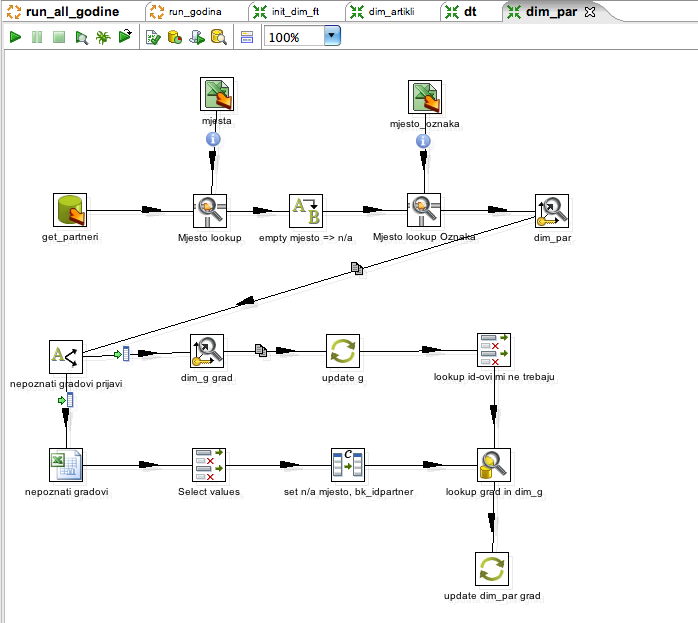
\includegraphics[width=15cm]{img/kettle_tr_dim_par.png}
\caption{Kettle transformacija: Generacija "dim\_par" i "dim\_g" `dimension' tabela za određenu poslovnu godinu}
\end{figure}

\begin{figure}[H]
\centering
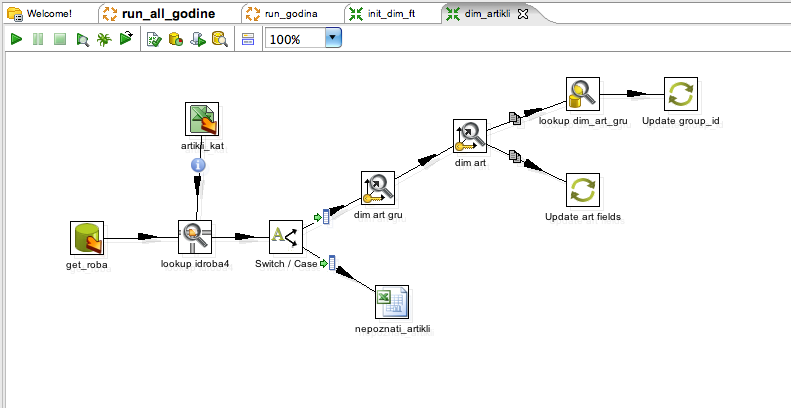
\includegraphics[width=15cm]{img/kettle_tr_dim_artikli.png}
\caption{Kettle transformacija: Generacija "dim\_art" i "dim\_art\_gru" `dimension' tabela za određenu poslovnu godinu}
\end{figure}


\begin{figure}[H]
\centering
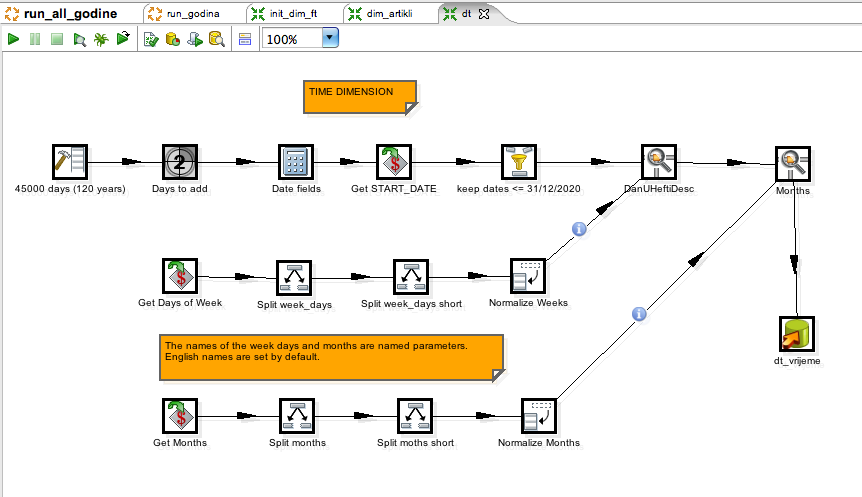
\includegraphics[width=15cm]{img/kettle_tr_dt.png}
\caption{Kettle transformacija: Generacija "dim\_dt" `dimension' tabele - vremenska dimenzija}
\end{figure}


\begin{figure}[H]
\centering
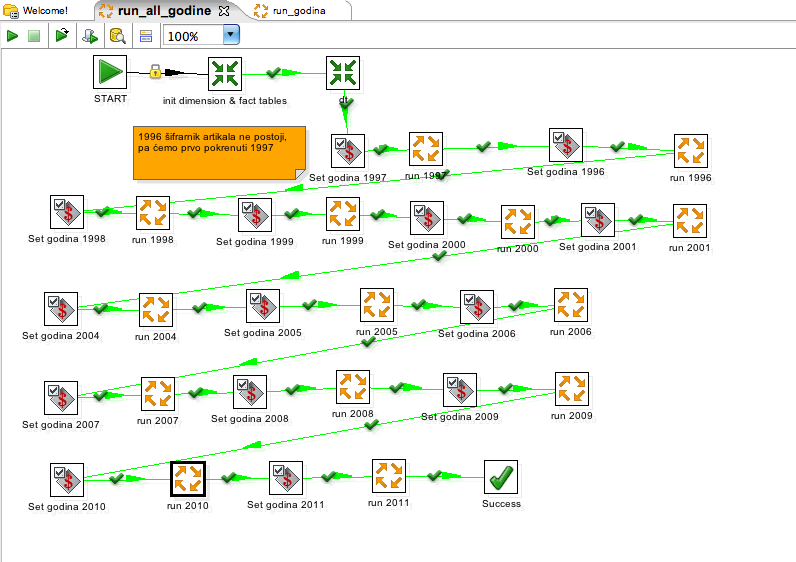
\includegraphics[width=15cm]{img/kettle_job_run_all.png}
\caption{Kettle job: inicijalizacija OLAP tabela, te generacija OLAP pdoataka za sve poslovne godine 1996-2011}
\end{figure}

\begin{figure}[H]
\centering
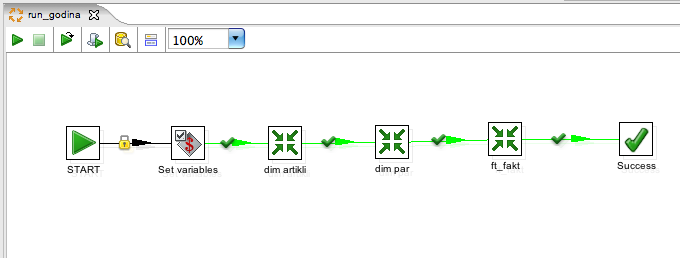
\includegraphics[width=15cm]{img/kettle_job_run_godina.png}
\caption{Kettle job: Generacija OLAP podataka iz F18 ERP izvora za jednu poslovnu godinu}
\end{figure}


\begin{figure}[H]
\centering
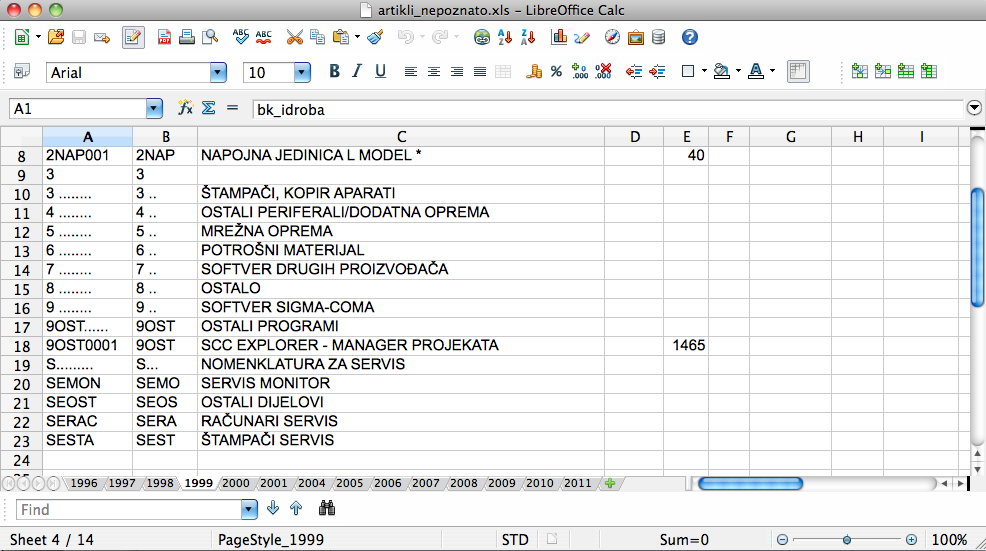
\includegraphics[width=15cm]{img/nepoznato_artikli.png}
\caption{Error reporting putem `spreadsheet' dokumenata - artikli za koje nisu definisani kodovi u olap\_cleansing tabelama}
\end{figure}

\begin{figure}[H]
\centering
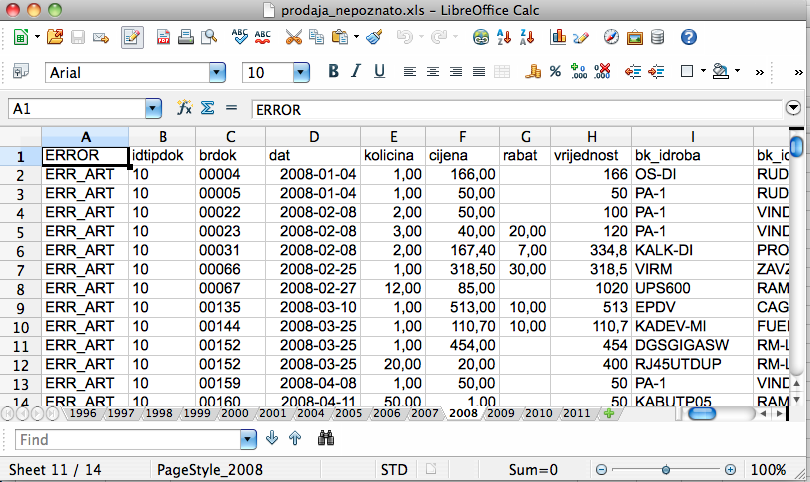
\includegraphics[width=15cm]{img/nepoznato_prodaja.png}
\caption{Dokumenti prodaje u kojima su neispravni podaci potrebni za popunjavanje dimension tabela (datum, klijent, roba) }
\end{figure}

\chapter{Iza case study-ja ?}

\section{Ne znam}

\subsection{Mondrian}

Snowflake mondrian - join

\cite{web:pentaho:mondrian_schema}

\subsection{datamart vs datawarehouse}

'Data mart' sadrži informacije o jednom dijelu organizacije (npr. prodaja, ljudski resursi), dok 'datawarehouse' sadrži informacije iz više područja -  obrađuje organizaciju globalno. 

'Data warehouse' je stoga usmjeren na podršku 'top' menadžmenta, dok 'datamart' obezbjeđuje informacije za upravljanje i operativno planiranje pojedinih dijelova organizacije  \cite[str.~391]{pentaho32}.

\subsection{Konstrukcija OLAP kocke}

surogat key (id)

business key (bk)

dimension table

facts table

SCD slow changing dimension
\begin{itemize}
  \item Type I
  \item Type II
\end{itemize}



\section{Pentaho}

Pentaho: analysis multidimensional, reporting, dashboards (key performance indicators) \cite[str.~7]{pentaho32}.

\begin{figure}[H]
\centering
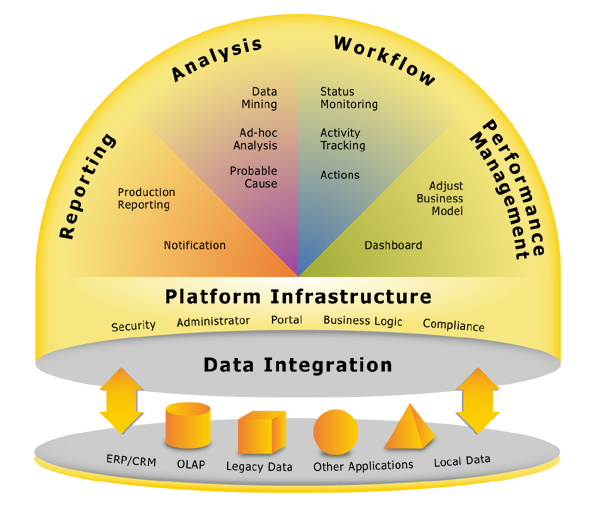
\includegraphics[width=15cm]{img/pentaho_arhitektura_eric.png}
\caption{Pentaho arhitektura (\cite{web:eric})}
\end{figure}



\section{Spoon}



\section{Data mining}

Data mining Weka projekat: \cite{web:weka}, \cite{web:pentaho_weka}

R statistički paket \cite{web:r}

\subsection{dimension table}

\begin{figure}[h]
\centering
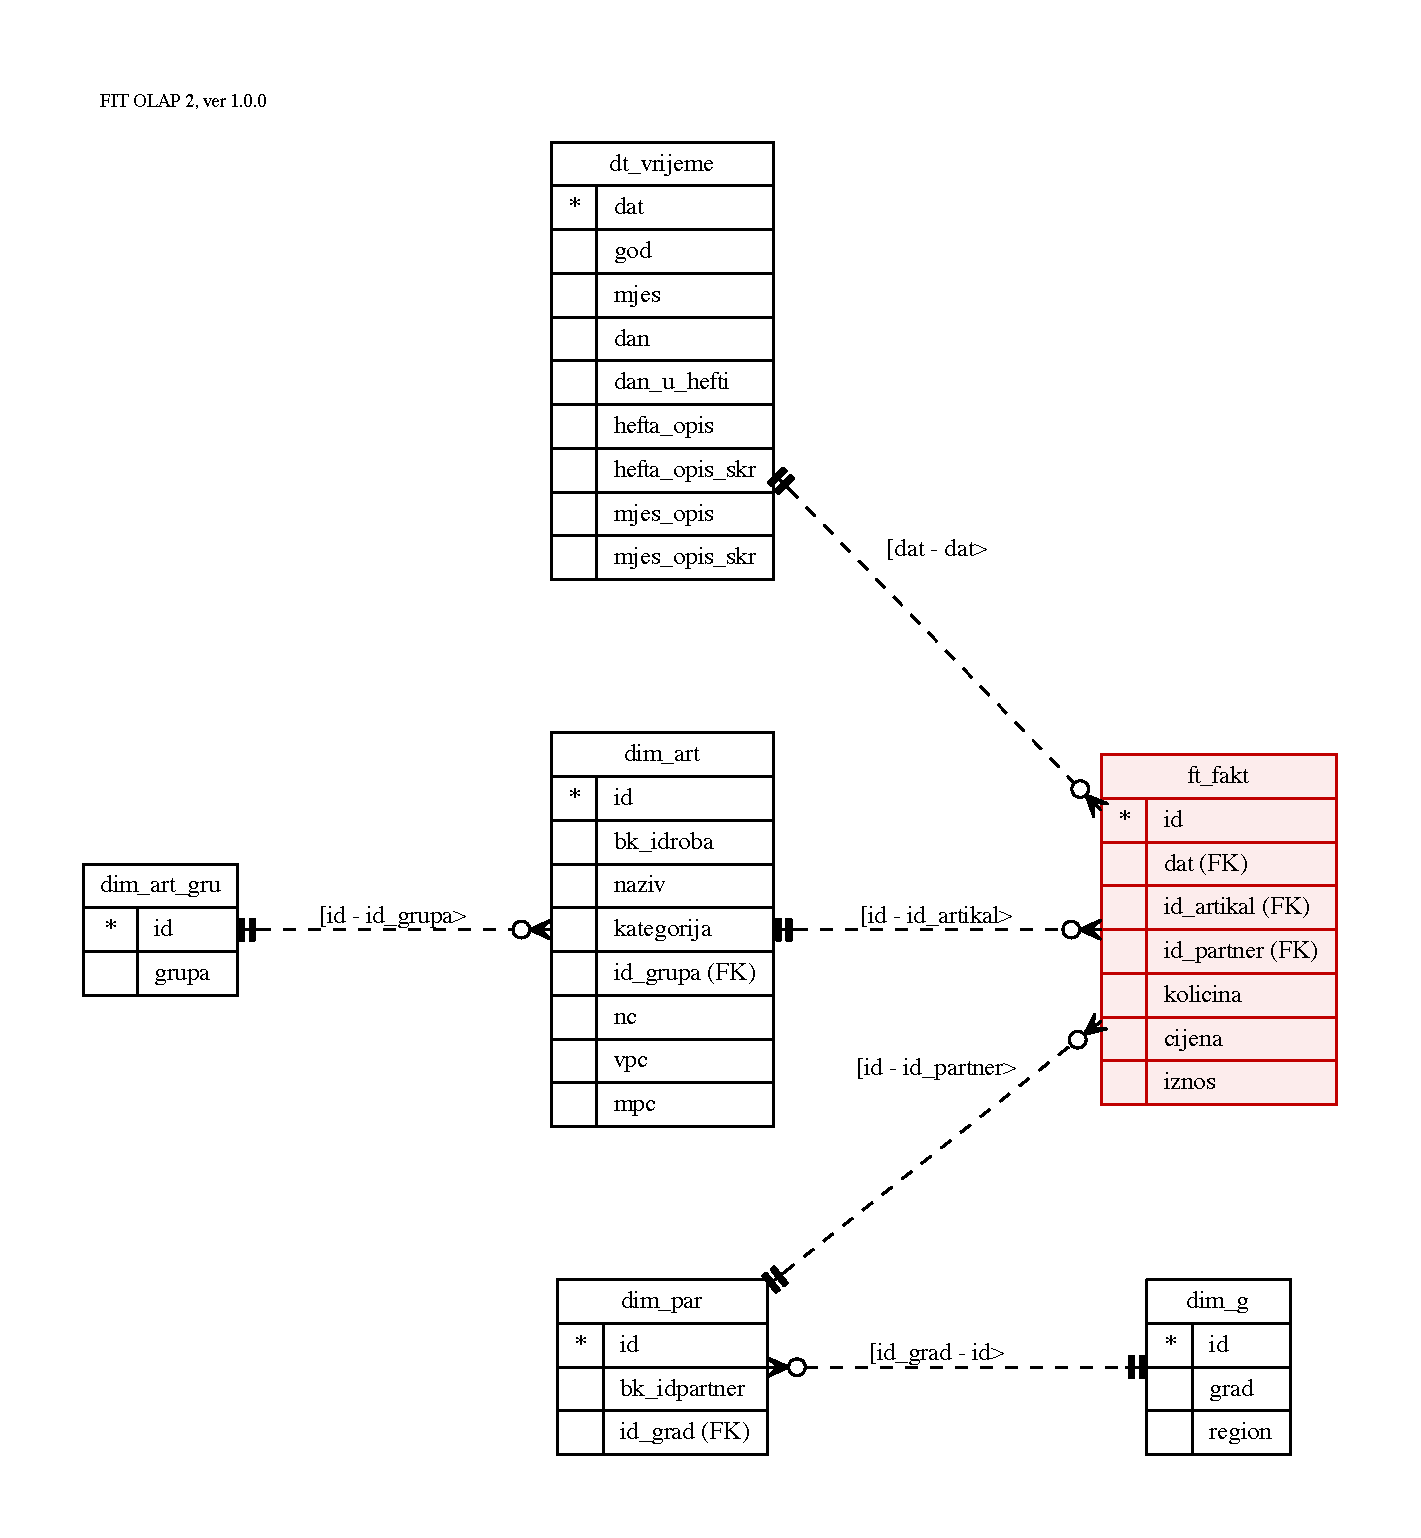
\includegraphics[width=15cm]{img/F18_olap.pdf}
\caption{OLAP schema}
\end{figure}


Mondrian schema:

\begin{figure}[h]
\centering
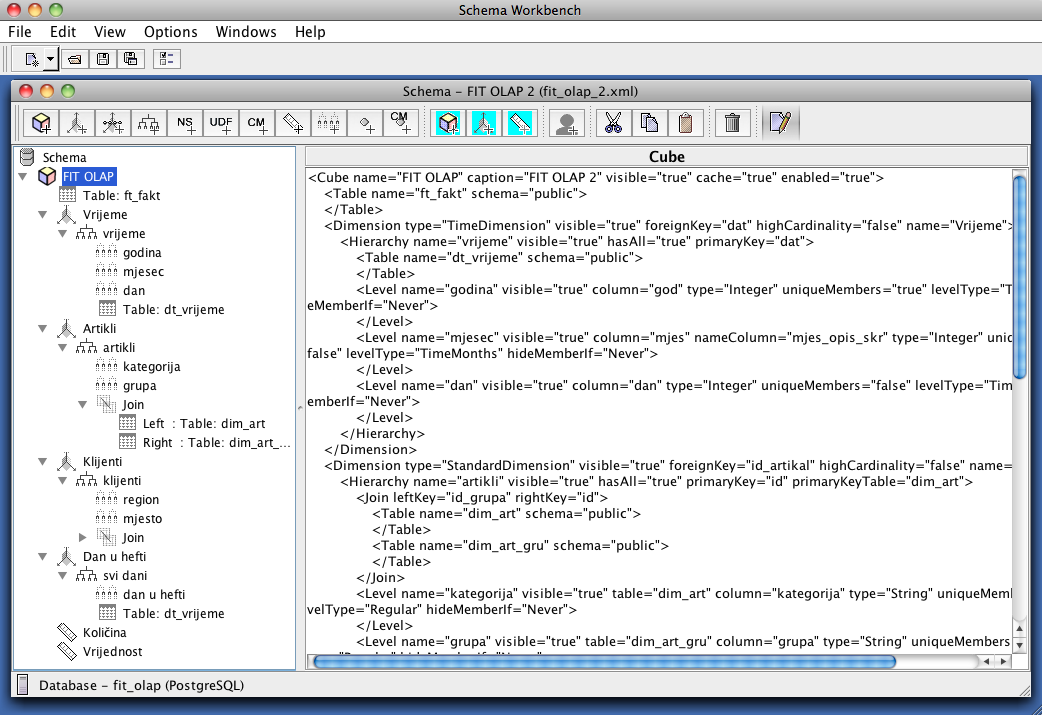
\includegraphics[width=15cm]{img/fit_olap_mondrian_schema}
\caption{Mondrian schema OLAP 2 cube}
\end{figure}




\subsection{facts table}



\subsection{ETL (Extract Transforn Load)}



\section{Poslovna pitanja (Business questions)}

Kolika je prodaja u određenom vremenskom periodu ?

Kakav je odnos prodaje prodaje za određeni period tekuće godine u odnosu na predhodne ?

Koji su efekti zapošljavanja radnika po pitanju ostvarnih prihoda ?


\section{Analiza podataka}

\lstset{ %
   language=SQL,
   basicstyle=\small,
   numbers=left,
   numbersep=5pt,
   breaklines=true,
   backgroundcolor=\color{yellow!15},
   tabsize=2,
   keywordstyle=\color{blue},
   captionpos=b, 
   frame=none
}


\begin{figure}[H]
\centering
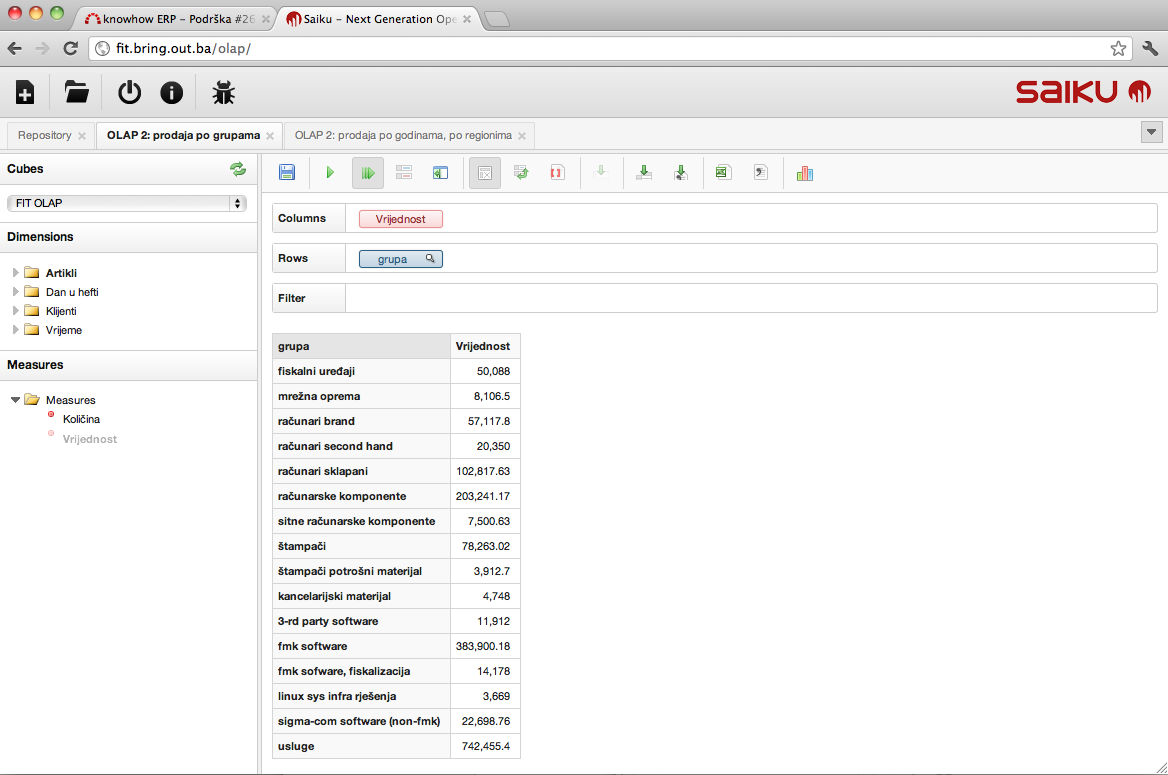
\includegraphics[width=15cm]{img/saiku_rpt_grupe}
\caption{Pregled prodaje po grupama artikala}
\end{figure}

\lstset{caption={Pregled prodaje po grupama artikala}}
\begin{lstlisting}
SELECT
NON EMPTY {Hierarchize({[Measures].[Vrijednost]})} 
ON COLUMNS,
  NON EMPTY {Hierarchize({[Artikli.artikli].[grupa].Members})} 
ON ROWS
FROM [FIT OLAP]
WHERE {Hierarchize({[Vrijeme.vrijeme].[All Vrijeme.vrijemes]})}
\end{lstlisting}


\begin{figure}[H]
\centering
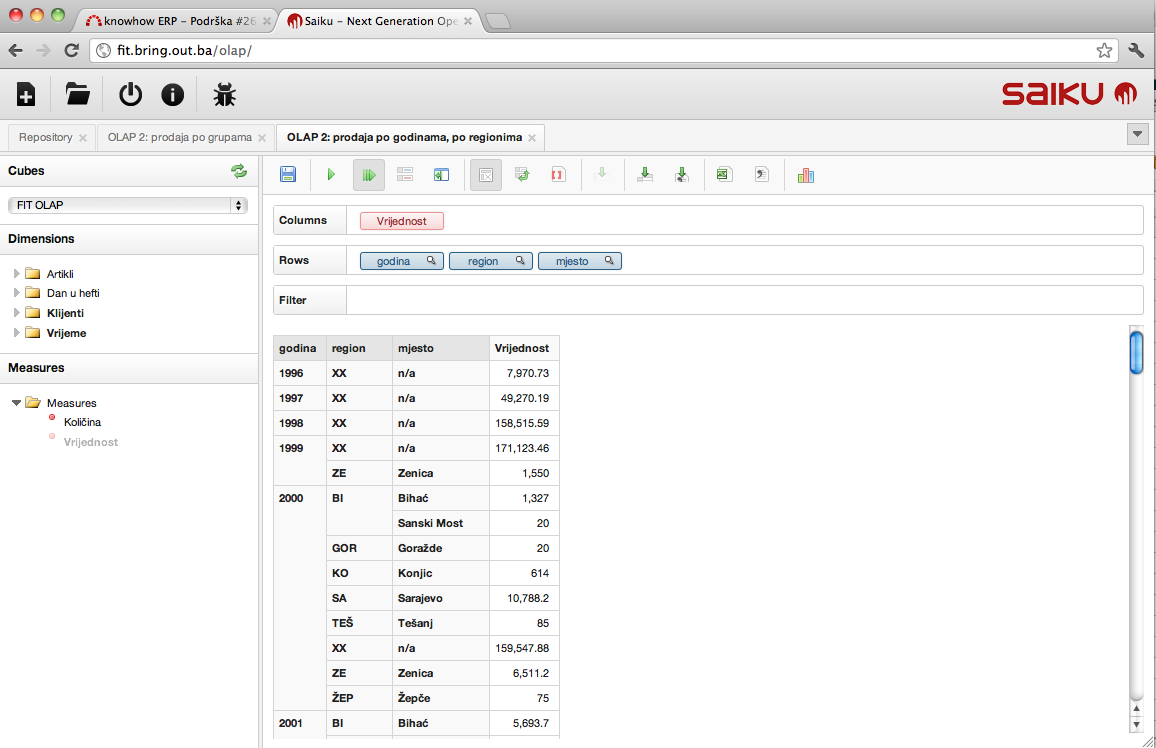
\includegraphics[width=15cm]{img/saiku_rpt_region}
\caption{Pregled prodaje po regionima, po godinama}
\end{figure}

\lstset{caption={Pregled prodaje po regionima}}
\begin{lstlisting}
SELECT
  NON EMPTY {Hierarchize({[Measures].[Vrijednost]})} 
ON COLUMNS,
  NON EMPTY 
    Hierarchize(
      Union(CrossJoin([Vrijeme.vrijeme].[godina].Members, 
      [Klijenti.klijenti].[region].Members), CrossJoin([Vrijeme.vrijeme].[godina].Members, 
      [Klijenti.klijenti].[mjesto].Members))
    ) 
ON ROWS
FROM [FIT OLAP]
\end{lstlisting}


\subsection{Redovi, Kolone, Filteri}

objasniti OLAP analysis ...



\subsection{Ekspert}

Poznavanje sadržaja i postojećih struktura podataka.



navodim pentaho: \cite{pentaho32}

navodim stranu 215: \cite[str.~215]{pentaho32}

wikipedia olap cube: \cite{web:wikipedia:olap_cube}
wikipedia xmla: \cite{web:wikipedia:xmla}

\chapter{Zaključak}
Zaključak.

\bibliography{literatura}
\bibliographystyle{fit}

\chapter{Rezime}
Rezime.

\appendix

\chapter{Korišteni alati}

\chapter{Izvorni kod, dostupni resursi}
\label{chap:izvorni_kod}

\begin{enumerate}[labelindent=\parindent,leftmargin=*]
   \item OLAP mondrian, kettle transformacije i job-ovi, erviz modeli: \url{https://github.com/hernad/hello_bi}
   \item Latex kod ovog dokumenta \url{https://github.com/hernad/MIS/tree/master/latex}
   \item olap\_cleansing `spreadsheet' dokument \url{https://github.com/hernad/hello_bi/raw/master/olap_cleansing.xls}
   \item Saiku demo server online: \url{http://fit.bring.out.ba/olap/#}
\end{enumerate}

\chapter{Bilješke autora}

\begin{enumerate}
  \item Prva verzija ovog seminarskog rada, neuspješno \url{https://github.com/hernad/MIS/raw/master/knowhowERP_OLAP_blog_style.pdf}
  \item FIT OLAP 2 cube: \url{http://redmine.bring.out.ba/issues/26711}
\end{enumerate}

\end{document}
